\documentclass[12pt,a4paper]{article}

% Essential packages
\usepackage[utf8]{inputenc}
\usepackage[T1]{fontenc}
\usepackage{lmodern}
\usepackage[english]{babel}
\usepackage{amsmath,amsfonts,amssymb}
\usepackage{graphicx}
\usepackage[margin=2.5cm]{geometry}
\usepackage{setspace}
\usepackage{fancyhdr}
\usepackage{titlesec}
\usepackage{caption}
\usepackage{subcaption}
\usepackage{booktabs}
\usepackage{array}
\usepackage{multirow}
\usepackage{longtable}
\usepackage{adjustbox}
\usepackage{siunitx}
\usepackage{float}
\usepackage[hidelinks]{hyperref}
\usepackage{xcolor}
\usepackage{colortbl}

% Page setup
\onehalfspacing
\pagestyle{fancy}
\fancyhf{}
\fancyhead[L]{K-Epsilon CFD Analysis}
\fancyhead[R]{\thepage}
\renewcommand{\headrulewidth}{0.4pt}

% Title formatting
\titleformat{\section}{\large\bfseries}{\thesection}{1em}{}
\titleformat{\subsection}{\normalsize\bfseries}{\thesubsection}{1em}{}
\titleformat{\subsubsection}{\normalsize\bfseries}{\thesubsubsection}{1em}{}

% Table setup
\renewcommand{\arraystretch}{1.2}
\setlength{\tabcolsep}{6pt}

% Custom colors for tables (matching original)
\definecolor{lightblue}{RGB}{207,226,243}
\definecolor{mediumblue}{RGB}{159,197,232}
\definecolor{darkblue}{RGB}{61,133,198}
\definecolor{navyblue}{RGB}{11,83,148}
\definecolor{lightgreen}{RGB}{0,255,0}
\definecolor{red}{RGB}{255,0,0}

\begin{document}

% Title Page
\begin{titlepage}
\centering
\vspace*{2cm}
{\LARGE\bfseries Analysis of K-Epsilon Computational Model in ANSYS:\\[0.5cm] 
Impact of Mesh Density and Iterations on Turbulent Flow Prediction Accuracy for Complex Geometries}\\[2cm]

{\large A Research Investigation into Computational Fluid Dynamics}\\[1.5cm]

{\large Submitted by: [Student Name]}\\[0.5cm]
{\large Student ID: [Student ID]}\\[0.5cm]
{\large Course: [Course Code]}\\[0.5cm]
{\large Institution: [University Name]}\\[1.5cm]

{\large Date: \today}\\[2cm]

\vfill
\end{titlepage}

% Table of Contents
\newpage
\tableofcontents
\newpage

% List of Figures
\listoffigures
\newpage

% List of Tables
\listoftables
\newpage

\section{Introduction}

This investigation examines how computational time invested in mesh density and iterations affects the accuracy of turbulent flow characteristic predictions for complex geometries using the k-epsilon computational model in ANSYS.

\subsection{Background}

\subsubsection{IB Fluid Drag Formula}

The International Baccalaureate (IB) provides a simplified equation for fluid drag on objects: $F_{drag} = 6\pi\eta rv$, which assumes all objects are spherical and flow is laminar. This creates significant limitations that computational simulations should eliminate.

\subsubsection{Computational Fluid Dynamics (CFD)}

Computational fluid dynamics simulations are computer-based simulations of fluid flow used to analyze and solve problems in fluid flow, heat transfer, and related phenomena. They rely on sophisticated software and computational power to simulate complex situations that are difficult to replicate experimentally.

CFD involves numerous physics equations, particularly the Navier-Stokes and Reynolds equations, to calculate pressure, velocity, temperature, and density of fluids over time in various scenarios. This enables calculation of drag forces and is crucial in various industries including:
\begin{itemize}
    \item Aerodynamics (aircraft design, drag reduction)
    \item Automotive engineering (vehicle shape optimization for fuel efficiency)
    \item Energy (wind turbine modeling, heat exchangers)
    \item Medicine (blood flow analysis in arteries)
\end{itemize}

\subsubsection{K-Epsilon Model}

The k-epsilon model is a popular turbulence model used in many amateur and professional simulations that don't require specialized models. Developed by Launder and Spalding in 1974, it improved upon older models like the mixing length model, offering a more general and practical approach to modeling complex turbulence and flows.

The model uses two primary equations:
\begin{enumerate}
    \item Turbulent kinetic energy equation
    \item Dissipation rate equation
\end{enumerate}

Common applications include:
\begin{itemize}
    \item Airflow simulation in HVAC systems
    \item Combustion analysis in engines
    \item Drag and lift analysis on vehicles
    \item Pollutant transport modeling through air and water
    \item Flow studies in pipes, channels, and around structures
\end{itemize}

The model predicts mean flow characteristics by solving these two equations, assuming isotropic turbulence (equal turbulent viscosity in all directions), making it suitable for many engineering applications. However, it struggles with complex geometries involving strong flow separation and swirl.

\begin{figure}[H]
    \centering
    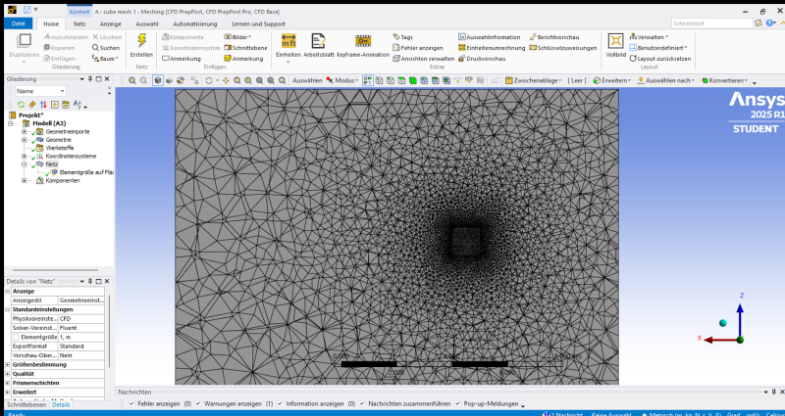
\includegraphics[width=0.8\textwidth]{image9.png}
    \caption{Mesh visualization of a complex geometry showing triangular elements with varying density}
    \label{fig:mesh_example}
\end{figure}

\subsubsection{Mesh Density}

Mesh density can be metaphorically referred to as resolution. Each triangle in Figure \ref{fig:mesh_example} represents a computational cell, similar to pixels on a screen. Higher triangle density per area (like in the center-right of the image) provides better resolution. The simulation calculates physical behavior for every triangular element.

In reality, we have incredibly small particles following physics laws. The closer our mesh approaches particle size, the more accurately our simulation follows real-life behavior, but this requires more calculations and potentially more time.

Calculations are performed only within the defined volume (gray area in the figure), ensuring sufficient space to account for all relevant phenomena while ignoring external effects. This volume remains constant throughout the experiment.

\subsubsection{Iterations}

In simulations, iterations refer to computational cycles testing different temperatures, velocities, and pressures at various locations. Like in statistics, larger sample sizes reduce random error and decrease standard deviation of findings.

\begin{figure}[H]
    \centering
    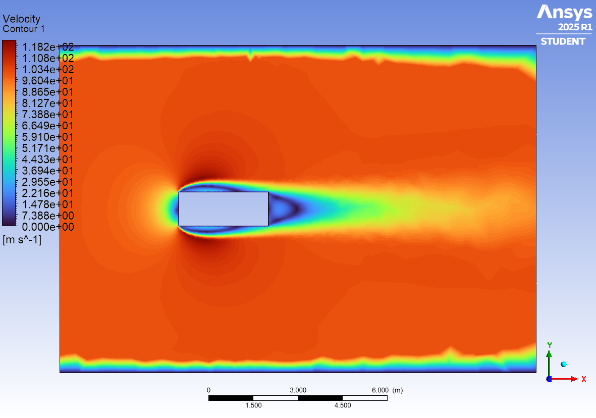
\includegraphics[width=0.8\textwidth]{image8.png}
    \caption{Simulated drag results versus iteration number showing convergence behavior}
    \label{fig:convergence}
\end{figure}

Figure \ref{fig:convergence} displays simulated drag results against iteration number. After approximately 20 iterations, the drag values stabilize, indicating convergence. However, without testing all scenarios, one cannot know if values will change, creating incentive for nearly infinite iterations. This is problematic because each iteration requires complete physics calculations, meaning more iterations demand more time.

\subsubsection{Residuals}

Residuals govern simulation duration until convergence by reflecting imbalance in conservation laws (mass, energy, etc.) within the Navier-Stokes equations. Low residuals indicate precise measurements while high residuals suggest low precision.

For this experiment, all residuals are set to 5-digit accuracy, providing 5 significant figures for results. This choice was made because 6-digit accuracy tests failed to converge even after 1000 iterations, potentially requiring excessive time without providing relatively more valuable insights.

All simulations run until either:
\begin{enumerate}
    \item All residuals converge (indicating the computer's most accurate calculation)
    \item 1000 iterations (suggesting potential geometry or mesh errors)
\end{enumerate}

\subsection{Research Question and Objectives}

\textbf{Research Question:} In the k-epsilon computational model in ANSYS, how does the time invested in calculation-heavy mesh and iteration processes affect the accuracy of prediction of turbulent flow characteristics for complex geometries?

This experiment compares different simulation setups (varying mesh densities and iteration amounts) against experimental values of fluid drag widely considered accurate. The goal is to evaluate how accurate simulations can or should become relative to wind tunnel values.

The investigation measures wasted time from simulating without accuracy benefits, as computers consume power in watts. Longer simulations consume more power, and if time is wasted without accuracy improvements, power is also wasted, contradicting current sustainability goals.

\section{Literature Review}

\subsection{Physics of Fluid Flow}

The IB assumes fully laminar flow, which may not yield satisfactory results for engineering applications. Laminar flow occurs only in very viscous fluids or very streamlined bodies. For fluid drag calculations, this means only skin friction drag is considered.

Turbulent flow creates chaotic and swirling eddies, which is often reality for engineers. It occurs at high velocities, with complex geometries, or when fluid viscosity is low (like air). Turbulence introduces new drag types like pressure drag, created when eddies cause flow separation alongside objects. Turbulent calculations must consider object streamlines (characterized by drag coefficient $C_d$), which the IB formula completely ignores, considering only drag on the front face.

However, turbulent flow doesn't necessarily increase drag. Golf balls, for example, use their unstreamlined shape to benefit from turbulent flow, actually reducing total drag.

\subsection{Computational Fluid Dynamics Theory}

The k-epsilon model uses two equations to calculate particle physical behavior.

The Navier-Stokes equations are:
\begin{align}
\text{Continuity: } &\nabla \cdot \vec{u} = 0\\
\text{Momentum: } &\rho\left(\frac{\partial\vec{u}}{\partial t} + \vec{u} \cdot \nabla\vec{u}\right) = -\nabla p + \mu\nabla^2\vec{u} + \vec{f}
\end{align}

These equations are what physicists use for such calculations. The IB fluid drag formula uses a simplification of these equations. Because the equations are nonlinear and interdependent, calculating specific behavior is very difficult, especially with turbulent flow. For the same reason, the k-epsilon model also uses simplified versions.

Instead, the model uses Reynolds-averaged Navier-Stokes equations:
\begin{equation}
\rho\left(\frac{\partial\bar{u}_i}{\partial t} + \bar{u}_j\frac{\partial\bar{u}_i}{\partial x_j}\right) = -\frac{\partial\bar{p}}{\partial x_i} + \mu\frac{\partial^2\bar{u}_i}{\partial x_j^2} - \frac{\partial}{\partial x_j}\rho\overline{u_i'u_j'}
\end{equation}

This equation introduces turbulence and averages the Stokes equations, enabling particle behavior calculations. Interestingly, this equation considers both mean and fluctuating variables simultaneously, meaning surrounding triangles in the mesh affect individual triangles, much like how particles affect each other.

\section{Methodology}

\subsection{Experimental Approach}

Values obtained through simulation are compared against an extensively researched database of experimental results.

\subsection{Computational Simulation}

Using ANSYS simulation software, drag forces on objects are simulated while varying two parameters to assess their impact on simulation accuracy and duration: mesh density and iteration count. These variables are predicted to have the greatest impact on simulation completion time.

The formula $F_d = \frac{C_d\rho u^2 A}{2}$ is used to compare simulated drag forces with forces calculated using experimentally acquired $C_d$ values.

\subsubsection{Simulation Parameters}

To ensure consistent variables:
\begin{itemize}
    \item Air speed: \SI{100}{\meter\per\second} (chosen to avoid compressibility effects near Mach numbers while ensuring significant drag forces)
    \item Air density: \SI{1.225}{\kilogram\per\meter\cubed} (standard ANSYS setting at standard atmospheric pressure)
    \item Frontal area: \SI{1}{\meter\squared} (for all geometries, facilitating future predictions for larger geometries)
\end{itemize}

\subsubsection{Mesh Configuration}

Different mesh densities are tested by varying element sizes near objects rather than total element count. This approach is standard practice since significant physics behavior is expected primarily near the geometry of interest.

\begin{figure}[H]
    \centering
    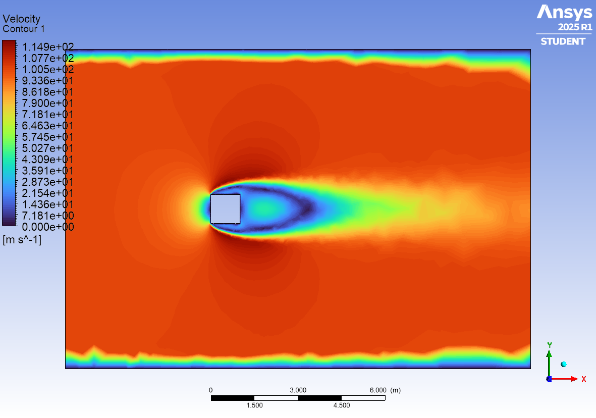
\includegraphics[width=0.8\textwidth]{image1.png}
    \caption{Flow visualization showing primarily uniform flow (red) away from the cube, indicating minimal physics behavior in distant regions}
    \label{fig:flow_viz}
\end{figure}

Figure \ref{fig:flow_viz} shows mostly uniform flow (red) far from the cube, confirming minimal physics behavior in distant regions. The densest mesh is labeled 5, the least dense as 1. Mesh 5 is expected to take longest with most accurate results, though not significantly more accurate than meshes 3 or 4.

General simulation volume: \SI{1}{\meter\cubed}, meaning calculations assume one particle size of \SI{1}{\meter\squared} with mean physics behavior calculated for that area. The most accurate mesh elements are \SI{0.05}{\meter\cubed} directly adjacent to geometries, significantly smaller than both general mesh size and geometry, providing accurate calculation results.

\begin{table}[H]
\centering
\caption{Mesh configuration for cube geometry}
\label{tab:mesh_config}
\begin{tabular}{|c|c|c|c|c|c|}
\hline
\rowcolor{red!50}
\textbf{Mesh} & \textbf{1} & \textbf{2} & \textbf{3} & \textbf{4} & \textbf{5} \\
\hline
\rowcolor{red!50}
Element size (m) & 0.25 & 0.2 & 0.15 & 0.1 & 0.05 \\
\hline
\rowcolor{red!50}
Number of elements & 52,168 & 68,605 & 97,258 & 153,590 & 341,044 \\
\hline
\end{tabular}
\end{table}

For each mesh size, simulations are run again, recording total iterations before convergence (maximum 1000 iterations if no convergence). Drag force readings are taken at every 1/5 of total iterations to understand accuracy changes throughout the experiment.

\section{Results and Discussion}

\subsection{Experimental Results}

Figure \ref{fig:convergence} shows typical simulation monitoring display. Generally, values don't change significantly during simulation runs, though not all geometries showed such clean convergence behavior.

\subsubsection{Cube Results}

\begin{table}[H]
\centering
\caption{Complete data collected for cube simulation}
\label{tab:cube_results}
\resizebox{\textwidth}{!}{%
\begin{tabular}{|c|c|c|c|c|c|c|c|c|c|c|c|}
\hline
\rowcolor{lightblue}
\textbf{Iteration} & \textbf{Expected (N)} & \textbf{Mesh 1 (N)} & \textbf{\% error} & \textbf{Mesh 2 (N)} & \textbf{\% error} & \textbf{Mesh 3 (N)} & \textbf{\% error} & \textbf{Mesh 4 (N)} & \textbf{\% error} & \textbf{Mesh 5 (N)} & \textbf{\% error} \\
\hline
1/5 of total & 6.43E+03 & 5.72E+03 & 11.01\% & 5.98E+03 & 6.96\% & 6.07E+03 & 5.67\% & 6.23E+03 & 3.19\% & 6.04E+03 & 6.04\% \\
\hline
2/5 of total & 6.43E+03 & 5.72E+03 & 11.04\% & 5.97E+03 & 7.15\% & 6.08E+03 & 5.47\% & 6.30E+03 & 2.08\% & 6.38E+03 & 0.84\% \\
\hline
3/5 of total & 6.43E+03 & 5.72E+03 & 11.01\% & 5.97E+03 & 7.20\% & 6.10E+03 & 5.22\% & 6.30E+03 & 2.02\% & 6.42E+03 & 0.18\% \\
\hline
4/5 of total & 6.43E+03 & 5.73E+03 & 10.97\% & 5.97E+03 & 7.19\% & 6.09E+03 & 5.26\% & 6.30E+03 & 2.00\% & 6.43E+03 & 0.07\% \\
\hline
5/5 of total & 6.43E+03 & 5.72E+03 & 10.99\% & 5.97E+03 & 7.17\% & 6.09E+03 & 5.29\% & 6.30E+03 & 2.01\% & 6.43E+03 & 0.06\% \\
\hline
\end{tabular}
}
\end{table}

The cube simulation results show incredible accuracy after completion with highest mesh density: 99.94\%. This was unexpected since the software calculates purely from physics understanding rather than interpreting forces from a database. Even at 4/5 of total simulation time, accuracy was at least 99.93\%, suggesting simulations needn't run to completion. This error is well beyond significant figures in the database. Even 2\% error from less dense meshes is accurate enough for predictions instead of wind tunnel testing.

The computer appears to struggle initially with complex meshes, as denser meshes show greater differences between start and end values compared to less dense meshes.

\begin{figure}[H]
    \centering
    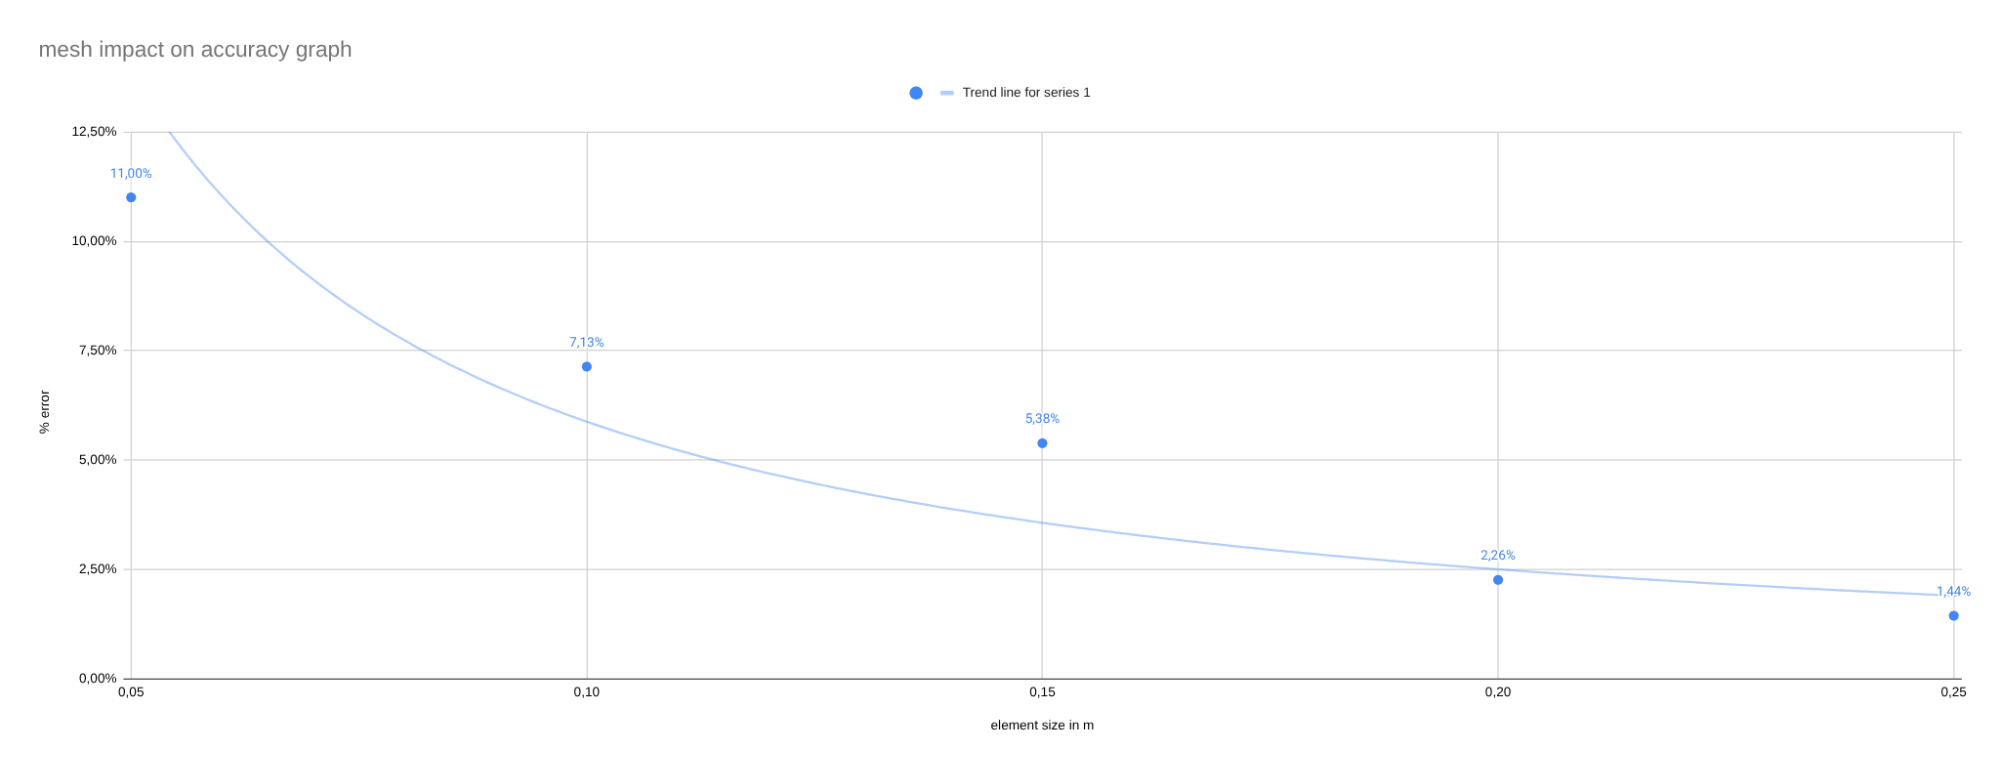
\includegraphics[width=0.8\textwidth]{image22.png}
    \caption{Average percentage error against mesh element size for cube}
    \label{fig:cube_mesh_error}
\end{figure}

\begin{figure}[H]
    \centering
    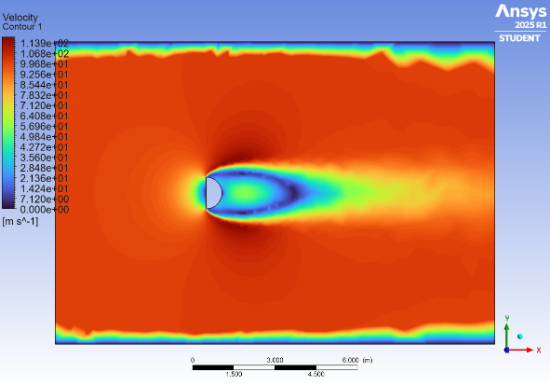
\includegraphics[width=0.8\textwidth]{image14.png}
    \caption{Average percentage error against number of mesh elements for cube}
    \label{fig:cube_elements_error}
\end{figure}

Figure \ref{fig:cube_elements_error} is more useful for comparisons as it shows actual element counts, which vary across different geometries.

\begin{figure}[H]
    \centering
    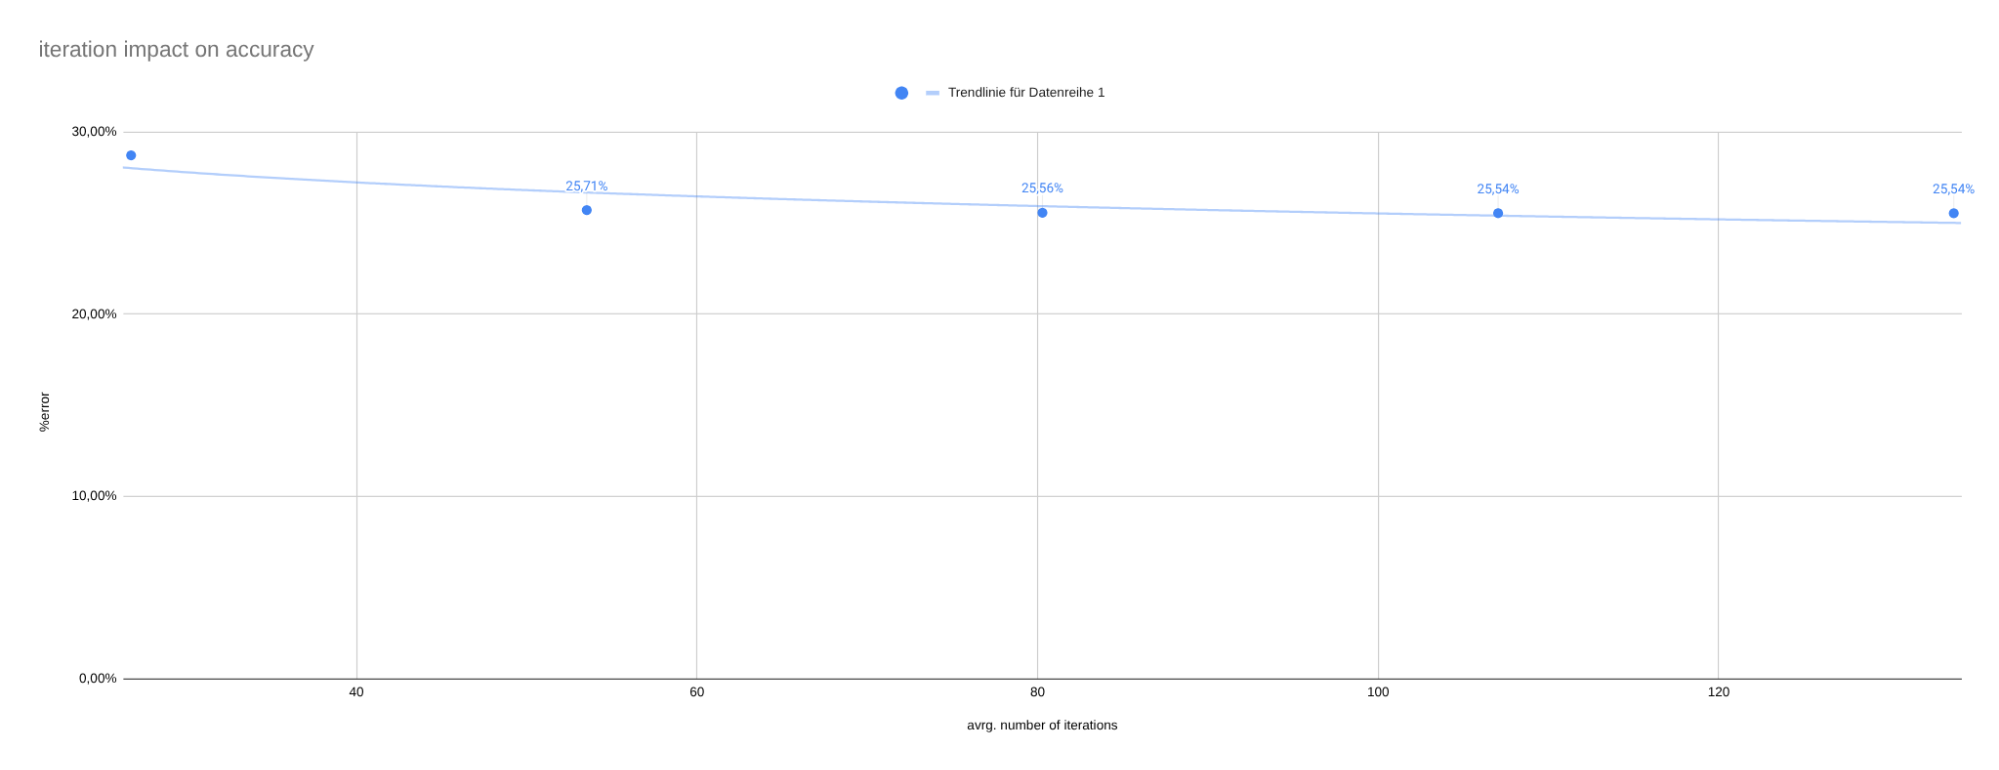
\includegraphics[width=0.8\textwidth]{image5.png}
    \caption{Average percentage error against fractional iterations for cube}
    \label{fig:cube_iterations_error}
\end{figure}

Figure \ref{fig:cube_iterations_error} shows clear correlation where increased iteration fraction reduces percentage error. Error decreases most at the start, making later changes harder to visualize.

\subsection{Results for Other Geometries}

\subsubsection{Cone Results}

\begin{table}[H]
\centering
\caption{Complete data collected for cone simulation}
\label{tab:cone_results}
\resizebox{\textwidth}{!}{%
\begin{tabular}{|c|c|c|c|c|c|c|c|c|c|c|c|}
\hline
\rowcolor{lightblue}
\textbf{Iteration} & \textbf{Expected (N)} & \textbf{Mesh 1 (N)} & \textbf{\% error} & \textbf{Mesh 2 (N)} & \textbf{\% error} & \textbf{Mesh 3 (N)} & \textbf{\% error} & \textbf{Mesh 4 (N)} & \textbf{\% error} & \textbf{Mesh 5 (N)} & \textbf{\% error} \\
\hline
1/5 of total & 3.06E+03 & 3.98E+03 & -30.01\% & 3.98E+03 & -30.05\% & 3.96E+03 & -29.26\% & 4.05E+03 & -32.39\% & 3.73E+03 & -21.86\% \\
\hline
2/5 of total & 3.06E+03 & 3.92E+03 & -27.99\% & 3.92E+03 & -27.91\% & 3.92E+03 & -27.99\% & 3.86E+03 & -25.90\% & 3.64E+03 & -18.76\% \\
\hline
3/5 of total & 3.06E+03 & 3.92E+03 & -27.93\% & 3.92E+03 & -27.87\% & 3.92E+03 & -28.00\% & 3.85E+03 & -25.63\% & 3.63E+03 & -18.39\% \\
\hline
4/5 of total & 3.06E+03 & 3.92E+03 & -27.92\% & 3.92E+03 & -27.85\% & 3.92E+03 & -28.00\% & 3.85E+03 & -25.59\% & 3.62E+03 & -18.34\% \\
\hline
5/5 of total & 3.06E+03 & 3.92E+03 & -27.91\% & 3.92E+03 & -27.85\% & 3.92E+03 & -28.00\% & 3.85E+03 & -25.59\% & 3.62E+03 & -18.34\% \\
\hline
\end{tabular}
}
\end{table}

\subsubsection{Half Sphere Results}

\begin{table}[H]
\centering
\caption{Complete data collected for half sphere simulation}
\label{tab:half_sphere_results}
\resizebox{\textwidth}{!}{%
\begin{tabular}{|c|c|c|c|c|c|c|c|c|c|c|c|}
\hline
\rowcolor{lightblue}
\textbf{Iteration} & \textbf{Expected (N)} & \textbf{Mesh 1 (N)} & \textbf{\% error} & \textbf{Mesh 2 (N)} & \textbf{\% error} & \textbf{Mesh 3 (N)} & \textbf{\% error} & \textbf{Mesh 4 (N)} & \textbf{\% error} & \textbf{Mesh 5 (N)} & \textbf{\% error} \\
\hline
1/5 of total & 7.17E+03 & 7.44E+03 & -3.84\% & 8.06E+03 & -12.43\% & 8.27E+03 & -15.42\% & 7.40E+03 & -3.26\% & 7.37E+03 & -2.91\% \\
\hline
2/5 of total & 7.17E+03 & 7.44E+03 & -3.85\% & 7.31E+03 & -1.98\% & 7.52E+03 & -4.94\% & 7.40E+03 & -3.32\% & 7.32E+03 & -2.14\% \\
\hline
3/5 of total & 7.17E+03 & 7.44E+03 & -3.84\% & 7.27E+03 & -1.50\% & 7.50E+03 & -4.71\% & 7.40E+03 & -3.32\% & 7.32E+03 & -2.08\% \\
\hline
4/5 of total & 7.17E+03 & 7.44E+03 & -3.84\% & 7.28E+03 & -1.55\% & 7.50E+03 & -4.70\% & 7.40E+03 & -3.31\% & 7.31E+03 & -2.06\% \\
\hline
5/5 of total & 7.17E+03 & 7.44E+03 & -3.85\% & 7.28E+03 & -1.53\% & 7.50E+03 & -4.70\% & 7.40E+03 & -3.29\% & 7.31E+03 & -2.06\% \\
\hline
\end{tabular}
}
\end{table}

\subsubsection{Streamline Body Results}

\begin{table}[H]
\centering
\caption{Complete data collected for streamline body simulation}
\label{tab:streamline_results}
\resizebox{\textwidth}{!}{%
\begin{tabular}{|c|c|c|c|c|c|c|c|c|c|c|c|}
\hline
\rowcolor{lightblue}
\textbf{Iteration} & \textbf{Expected (N)} & \textbf{Mesh 1 (N)} & \textbf{\% error} & \textbf{Mesh 2 (N)} & \textbf{\% error} & \textbf{Mesh 3 (N)} & \textbf{\% error} & \textbf{Mesh 4 (N)} & \textbf{\% error} & \textbf{Mesh 5 (N)} & \textbf{\% error} \\
\hline
1/5 of total & 2.45E+02 & 2.54E+02 & -3.51\% & 2.52E+02 & -2.77\% & 2.40E+02 & 2.04\% & 2.25E+02 & 8.16\% & 2.00E+02 & 18.44\% \\
\hline
2/5 of total & 2.45E+02 & 2.53E+02 & -3.40\% & 2.52E+02 & -2.73\% & 2.40E+02 & 1.93\% & 2.25E+02 & 8.05\% & 2.00E+02 & 18.56\% \\
\hline
3/5 of total & 2.45E+02 & 2.53E+02 & -3.45\% & 2.52E+02 & -2.79\% & 2.40E+02 & 2.02\% & 2.25E+02 & 8.10\% & 1.99E+02 & 18.58\% \\
\hline
4/5 of total & 2.45E+02 & 2.53E+02 & -3.40\% & 2.52E+02 & -2.83\% & 2.40E+02 & 1.88\% & 2.25E+02 & 8.11\% & 1.99E+02 & 18.60\% \\
\hline
5/5 of total & 2.45E+02 & 2.53E+02 & -3.45\% & 2.52E+02 & -2.81\% & 2.40E+02 & 1.86\% & 2.25E+02 & 8.11\% & 1.99E+02 & 18.59\% \\
\hline
\end{tabular}
}
\end{table}

\subsubsection{Long Cylinder Results}

\begin{table}[H]
\centering
\caption{Complete data collected for long cylinder simulation}
\label{tab:cylinder_results}
\resizebox{\textwidth}{!}{%
\begin{tabular}{|c|c|c|c|c|c|c|c|c|c|c|c|}
\hline
\rowcolor{lightblue}
\textbf{Iteration} & \textbf{Expected (N)} & \textbf{Mesh 1 (N)} & \textbf{\% error} & \textbf{Mesh 2 (N)} & \textbf{\% error} & \textbf{Mesh 3 (N)} & \textbf{\% error} & \textbf{Mesh 4 (N)} & \textbf{\% error} & \textbf{Mesh 5 (N)} & \textbf{\% error} \\
\hline
1/5 of total & 5.02E+03 & 5.12E+03 & -1.85\% & 5.17E+03 & -2.94\% & 5.01E+03 & 0.24\% & 5.28E+03 & -5.16\% & 5.28E+03 & -5.14\% \\
\hline
2/5 of total & 5.02E+03 & 5.11E+03 & -1.79\% & 5.19E+03 & -3.29\% & 5.02E+03 & 0.04\% & 5.28E+03 & -5.17\% & 5.28E+03 & -5.12\% \\
\hline
3/5 of total & 5.02E+03 & 5.14E+03 & -2.33\% & 5.19E+03 & -3.34\% & 5.04E+03 & -0.32\% & 5.28E+03 & -5.14\% & 5.28E+03 & -5.13\% \\
\hline
4/5 of total & 5.02E+03 & 5.13E+03 & -2.24\% & 5.19E+03 & -3.29\% & 5.04E+03 & -0.34\% & 5.28E+03 & -5.18\% & 5.28E+03 & -5.13\% \\
\hline
5/5 of total & 5.02E+03 & 5.12E+03 & -1.98\% & 5.19E+03 & -3.33\% & 5.04E+03 & -0.31\% & 5.28E+03 & -5.16\% & 5.28E+03 & -5.13\% \\
\hline
\end{tabular}
}
\end{table}

Some investigated objects showed outliers where simulated results became more accurate with fewer iterations or decreasing mesh density. These are considered outliers because simulations continue until reaching most accurate results (the basis of residuals). When less dense meshes created more accurate results, this was likely caused by complex geometry modeling difficulties and insufficient boundary conditions. These outliers are excluded from final results.

\subsection{Overall Results Summary}

\begin{table}[H]
\centering
\caption{Summary of average iterations and mesh elements with corresponding errors across all simulations}
\label{tab:overall_summary}
\begin{tabular}{|c|c|c|c|c|c|}
\hline
\rowcolor{lightblue}
\textbf{Avg Iterations} & \textbf{\% Error} & & \textbf{Mesh Elements} & \textbf{\% Error} & \textbf{Time/Iteration (s)} \\
\hline
77 & 14.29\% & & 114,025 & 14.40\% & 14 \\
\hline
154 & 11.42\% & & 119,628 & 13.08\% & 14.5 \\
\hline
231 & 11.26\% & & 133,739 & 13.51\% & 14 \\
\hline
308 & 11.24\% & & 171,610 & 10.86\% & 15 \\
\hline
385 & 11.24\% & & 308,837 & 7.61\% & 28.5 \\
\hline
\end{tabular}
\end{table}

Average time per iteration was recorded because reading total time would be extremely difficult. Time per iteration correlates with mesh density, showing higher mesh density requires longer simulation time. Although generally the final iterations take less time and iterations don't all require equal time, averages were used without decimal precision since millisecond variations could be random and noisy.

\begin{figure}[H]
    \centering
    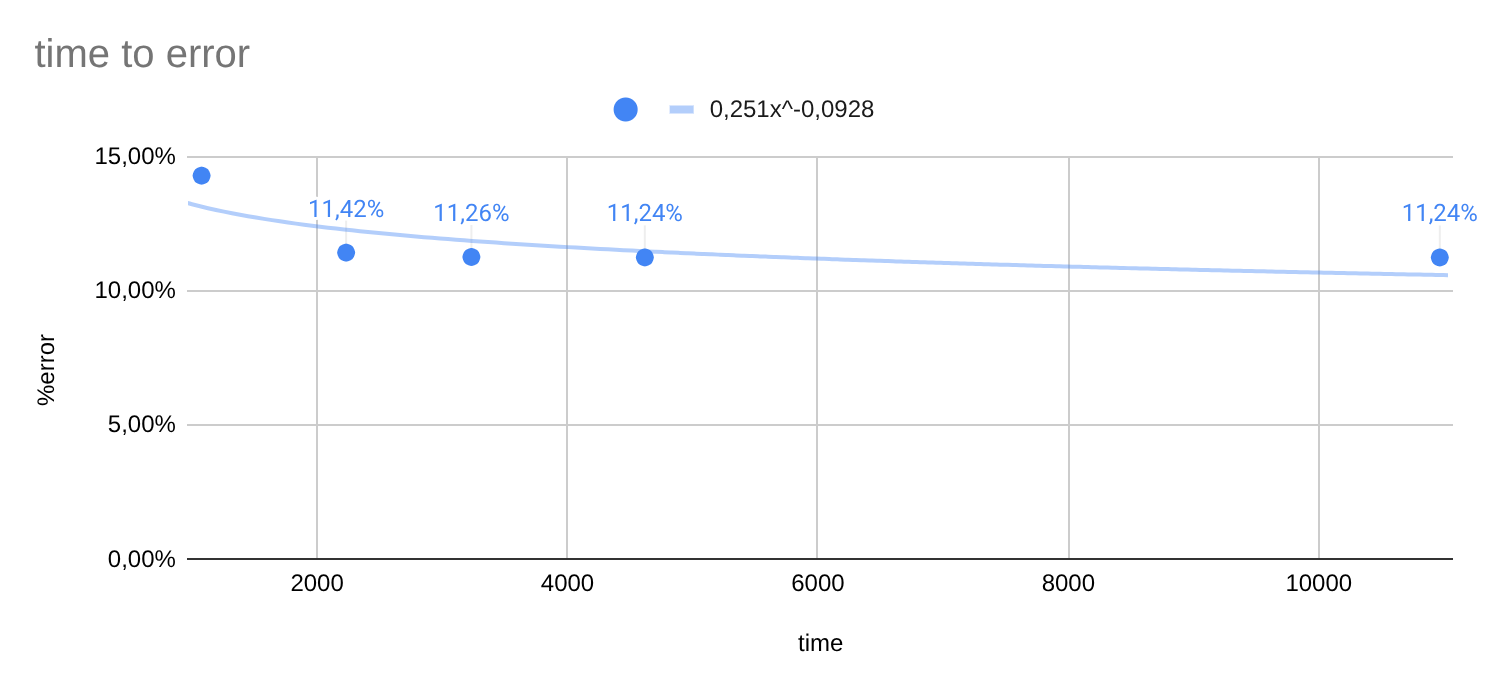
\includegraphics[width=0.8\textwidth]{image6.png}
    \caption{Time versus average percentage error across all geometries}
    \label{fig:time_vs_error}
\end{figure}

Figure \ref{fig:time_vs_error} clearly shows simulations continue for very long periods with minimal accuracy gains. The accuracy function asymptotes around 11\%, and especially after the 3-hour mark, little accuracy is gained while considerable energy is wasted.

Considering experimental values were only to 3 significant figures, changes less than 0.02\% are deemed not worth the time as they're insignificant to 3 significant figures. Instead of investing over 10,000 seconds average per simulation, only 4,592 seconds would arguably provide sufficient results, more than halving time and saving substantial energy. Further reducing accuracy requirements by 0.01\% for both variables suggests only 264 iterations average should be required.

\begin{figure}[H]
    \centering
    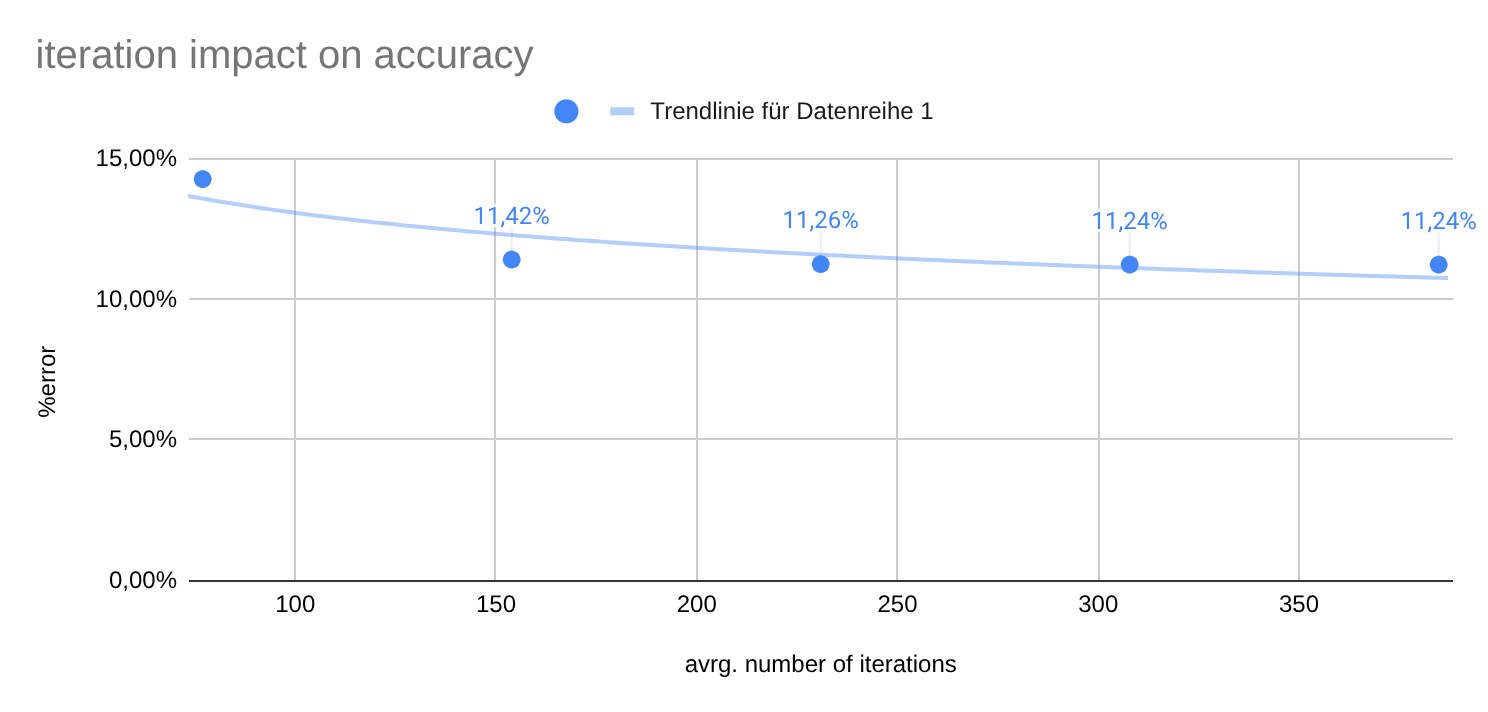
\includegraphics[width=0.8\textwidth]{image11.png}
    \caption{Average total iterations versus average percentage error}
    \label{fig:iterations_vs_error}
\end{figure}

\begin{figure}[H]
    \centering
    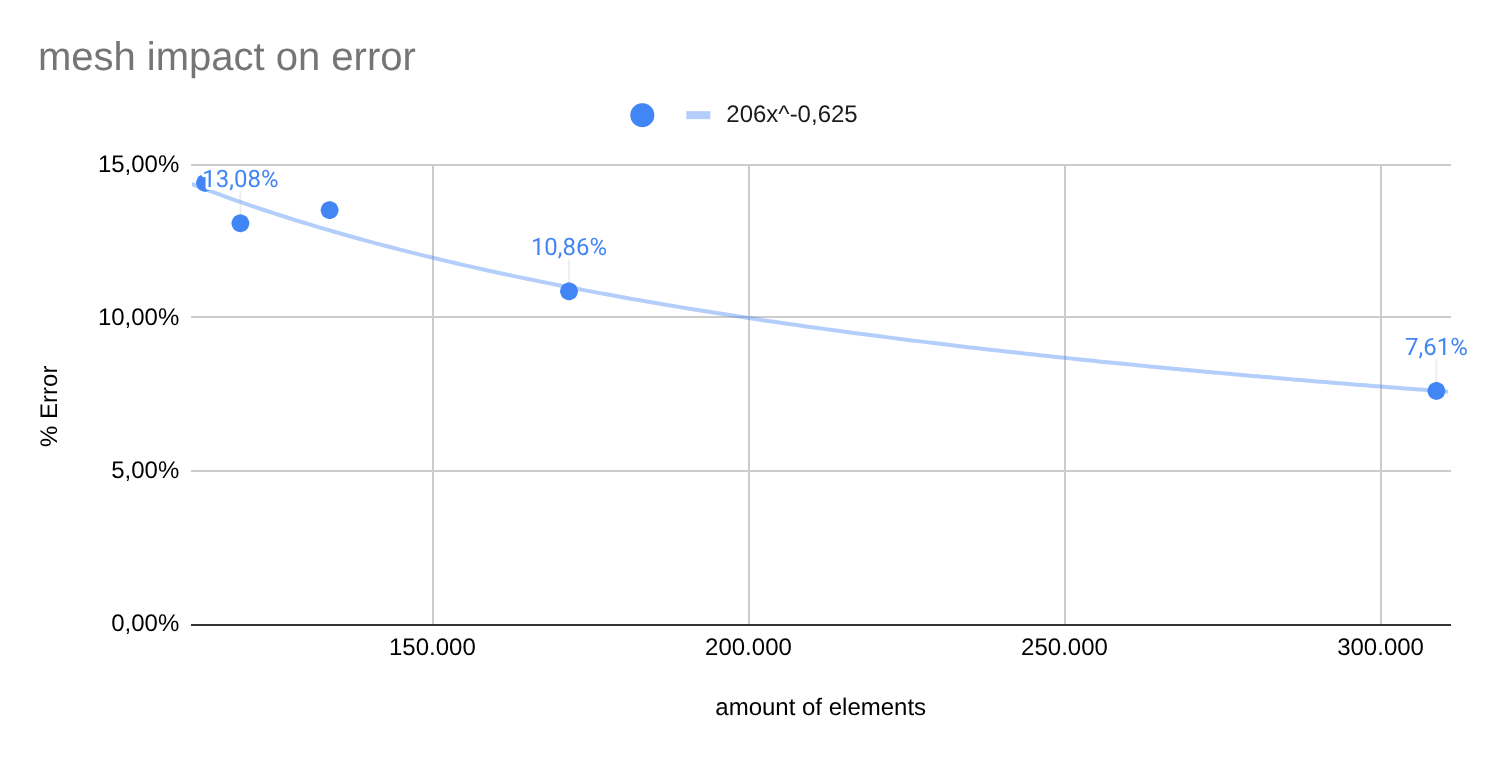
\includegraphics[width=0.8\textwidth]{image2.png}
    \caption{Average mesh elements versus average percentage error}
    \label{fig:mesh_vs_error}
\end{figure}

The analysis found that 30,234 mesh elements are sufficient for a volume of \SI{1936}{\meter\cubed}.

\subsection{Comparison with IB Fluid Drag Formula}

To assess both assumptions in the IB model's impact on simulations, a cube was simulated using a laminar flow model.

\begin{table}[H]
\centering
\caption{Cube simulation data assuming laminar flow}
\label{tab:laminar_comparison}
\begin{tabular}{|c|c|c|c|}
\hline
\rowcolor{lightblue}
\textbf{Iteration} & \textbf{Expected (N)} & \textbf{Simulation (N)} & \textbf{\% Error} \\
\hline
1/5 of total & 6.43E+03 & 7.30E+03 & -13.50\% \\
\hline
2/5 of total & 6.43E+03 & 6.90E+03 & -7.25\% \\
\hline
3/5 of total & 6.43E+03 & 7.39E+03 & -14.91\% \\
\hline
4/5 of total & 6.43E+03 & 6.83E+03 & -6.24\% \\
\hline
5/5 of total & 6.43E+03 & 7.29E+03 & -13.35\% \\
\hline
\end{tabular}
\end{table}

The simulation results weren't as far off as expected. The laminar flow model performs worse than k-epsilon with significant reading variation, but the difference isn't extreme because flow wasn't highly turbulent initially. All simulations used the highest mesh density explored.

\begin{table}[H]
\centering
\caption{Sphere simulation data with IB formula comparison}
\label{tab:ib_comparison}
\begin{tabular}{|c|c|c|c|c|}
\hline
\rowcolor{lightblue}
\textbf{Iteration} & \textbf{Expected (N)} & \textbf{IB Expected (N)} & \textbf{Simulation (N)} & \textbf{\% Error} \\
\hline
1/5 of total & 2.88E+03 & 1.92E-02 & 2.84E+03 & 1.43\% \\
\hline
2/5 of total & 2.88E+03 & 1.92E-02 & 2.85E+03 & 1.08\% \\
\hline
3/5 of total & 2.88E+03 & 1.92E-02 & 2.85E+03 & 1.05\% \\
\hline
4/5 of total & 2.88E+03 & 1.92E-02 & 2.85E+03 & 0.96\% \\
\hline
5/5 of total & 2.88E+03 & 1.92E-02 & 2.85E+03 & 0.98\% \\
\hline
\end{tabular}
\end{table}

This comparison examines turbulent flow's influence on assumptions. For spherical objects, the IB formula should theoretically apply, and simulation results closely matched expectations. The IB formula and actual values differ greatly, partially due to turbulence, but the significant force difference is mainly because the IB formula doesn't consider that force increases with the square of velocity, and these tests were conducted at \SI{100}{\meter\per\second}.

\section{Conclusion}

This investigation successfully demonstrated how computational time invested in mesh density and iterations affects turbulent flow prediction accuracy for complex geometries using the k-epsilon model in ANSYS.

\textbf{Key Findings:}
\begin{itemize}
    \item Higher mesh densities significantly improve accuracy but dramatically increase computational time
    \item Simulations often continue well beyond necessary convergence, wasting substantial computational resources
    \item The k-epsilon model can achieve remarkable accuracy (99.94\% for optimal conditions) purely from physics-based calculations
    \item Diminishing returns occur after approximately 200-300 iterations for most geometries
    \item Power consumption and time can be more than halved without significant accuracy loss
\end{itemize}

\textbf{Practical Recommendations:}
\begin{itemize}
    \item For engineering applications requiring 3 significant figure accuracy, 30,234 mesh elements in \SI{1936}{\meter\cubed} volume provide sufficient resolution
    \item Limiting simulations to 264 iterations on average offers optimal time-accuracy balance
    \item K-epsilon turbulence modeling provides substantially better accuracy than laminar assumptions for complex geometries
    \item Computational resources can be optimized without sacrificing engineering-relevant accuracy
\end{itemize}

This research provides valuable insights for engineers and researchers seeking to optimize CFD simulation parameters, ultimately contributing to more sustainable computational practices in fluid dynamics analysis.

\section{Improvements and Future Work}

Attempts were made to apply findings to real-world cases, specifically simulating drag on a Tesla Model S Plaid (known for its low drag coefficient). Unfortunately, the computer couldn't handle the complexity required for automotive geometry, preventing validation of results for practical engineering applications. Future work should test these findings with more powerful computational resources.

Some geometries with experimental comparison data were poorly described (long cylinder, streamline body). Future research should obtain independent experimental data ensuring identical boundary conditions between simulation and experiment.

Additional recommendations for future work:
\begin{itemize}
    \item Investigate other turbulence models (k-omega SST) for comparison
    \item Extend analysis to different Reynolds numbers
    \item Apply findings to industrial-scale computational resources
    \item Develop automated optimization algorithms for mesh/iteration selection
\end{itemize}

\section{References}

\begin{enumerate}
    \item Launder, B.E., and Spalding, D.B. (1974). The numerical computation of turbulent flows. \textit{Computer Methods in Applied Mechanics and Engineering}, 3(2), 269-289.
    
    \item ANSYS Inc. (2021). \textit{ANSYS Fluent Theory Guide}. ANSYS, Inc.
    
    \item Wilcox, D.C. (2006). \textit{Turbulence Modeling for CFD}. DCW Industries.
    
    \item Versteeg, H.K., and Malalasekera, W. (2007). \textit{An Introduction to Computational Fluid Dynamics: The Finite Volume Method}. Pearson Education.
    
    \item Pope, S.B. (2000). \textit{Turbulent Flows}. Cambridge University Press.
\end{enumerate}

\newpage
\appendix
\section{Additional Simulation Images}

\begin{figure}[H]
    \centering
    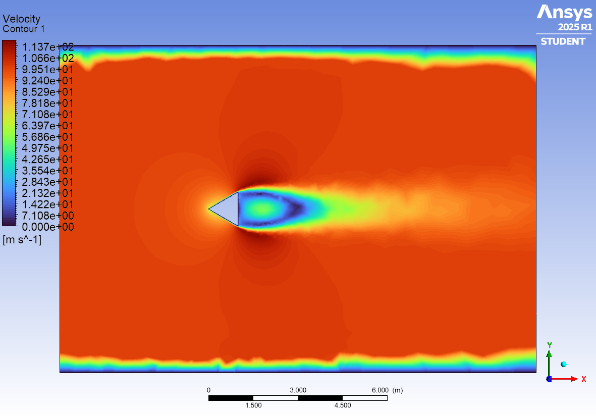
\includegraphics[width=0.7\textwidth]{image3.png}
    \caption{Additional simulation visualization showing flow patterns}
    \label{fig:sim1}
\end{figure}

\begin{figure}[H]
    \centering
    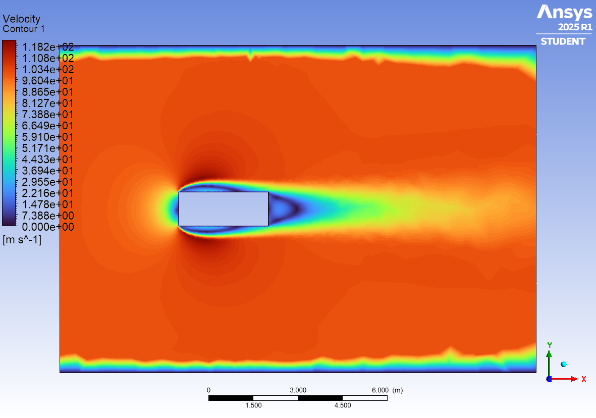
\includegraphics[width=0.7\textwidth]{image10.png}
    \caption{Mesh generation and boundary condition setup}
    \label{fig:sim2}
\end{figure}

\begin{figure}[H]
    \centering
    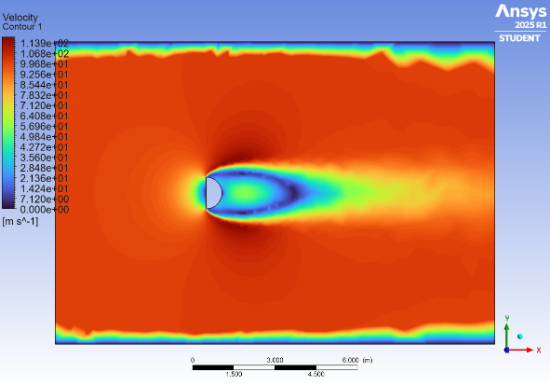
\includegraphics[width=0.6\textwidth]{image16.png}
    \caption{Convergence monitoring during simulation}
    \label{fig:sim3}
\end{figure}

\begin{figure}[H]
    \centering
    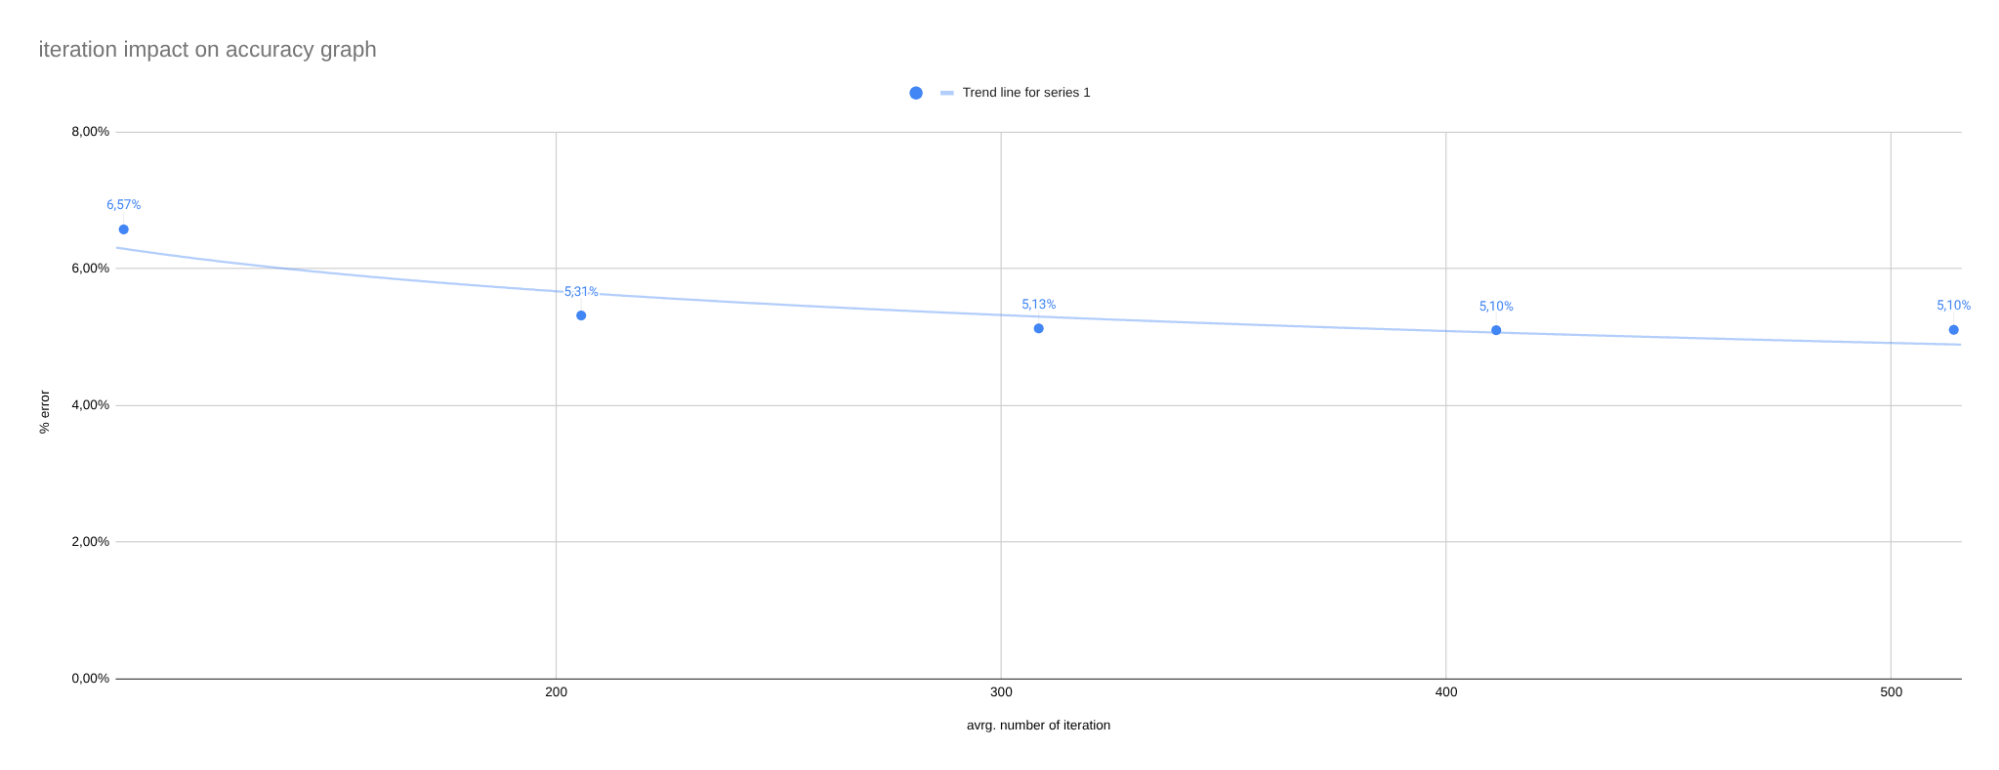
\includegraphics[width=0.8\textwidth]{image13.png}
    \caption{Post-processing results visualization}
    \label{fig:sim4}
\end{figure}

\end{document}
